\chapter{\IfLanguageName{dutch}{Opzetten van monolitische architectuur}{Setting up monolithic architecture}}
\label{ch:monoliet}
Er wordt begonnen met het opzetten van een ouderenboerderijapplicatie die een monolithische architectuur volgt, waarbij alle functionaliteiten zich binnen één enkele backend bevinden, wat zowel voordelen als beperkingen met zich meebrengt. In deze initiële opzet functioneert zowel de backend als de frontend elk op afzonderlijke poorten, met de backend volledig ontwikkeld in Node.js en de frontend in React. De communicatie tussen de backend en de MySQL-database gebeurt met Knex, terwijl de frontend via Axios API-calls met de backend communiceert, wat een gestroomlijnde interactie tussen de verschillende delen van de applicatie mogelijk maakt.

\begin{figure}[H]
	\centering	
	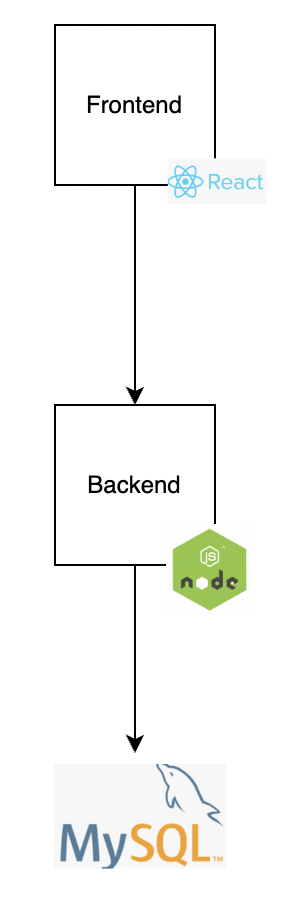
\includegraphics[width = 3cm]{monoliet.png} 
	\caption{Architectuur monolitische applicatie} 
	\label{fig:monolietBP} 
\end{figure}
\FloatBarrier


De functionaliteiten van de applicatie omvatten een auth0 inlogsysteem, een gebruikersprofielpagina en de mogelijkheid voor gebruikers om zich te registreren voor verschillende activiteiten. 

Bij het laden van de applicatie krijgt de gebruiker de homepagina te zien, waar hij wat infomatie over de boerderij en de activiteieten kan vinden.

\begin{figure}[H]
    \centering	
    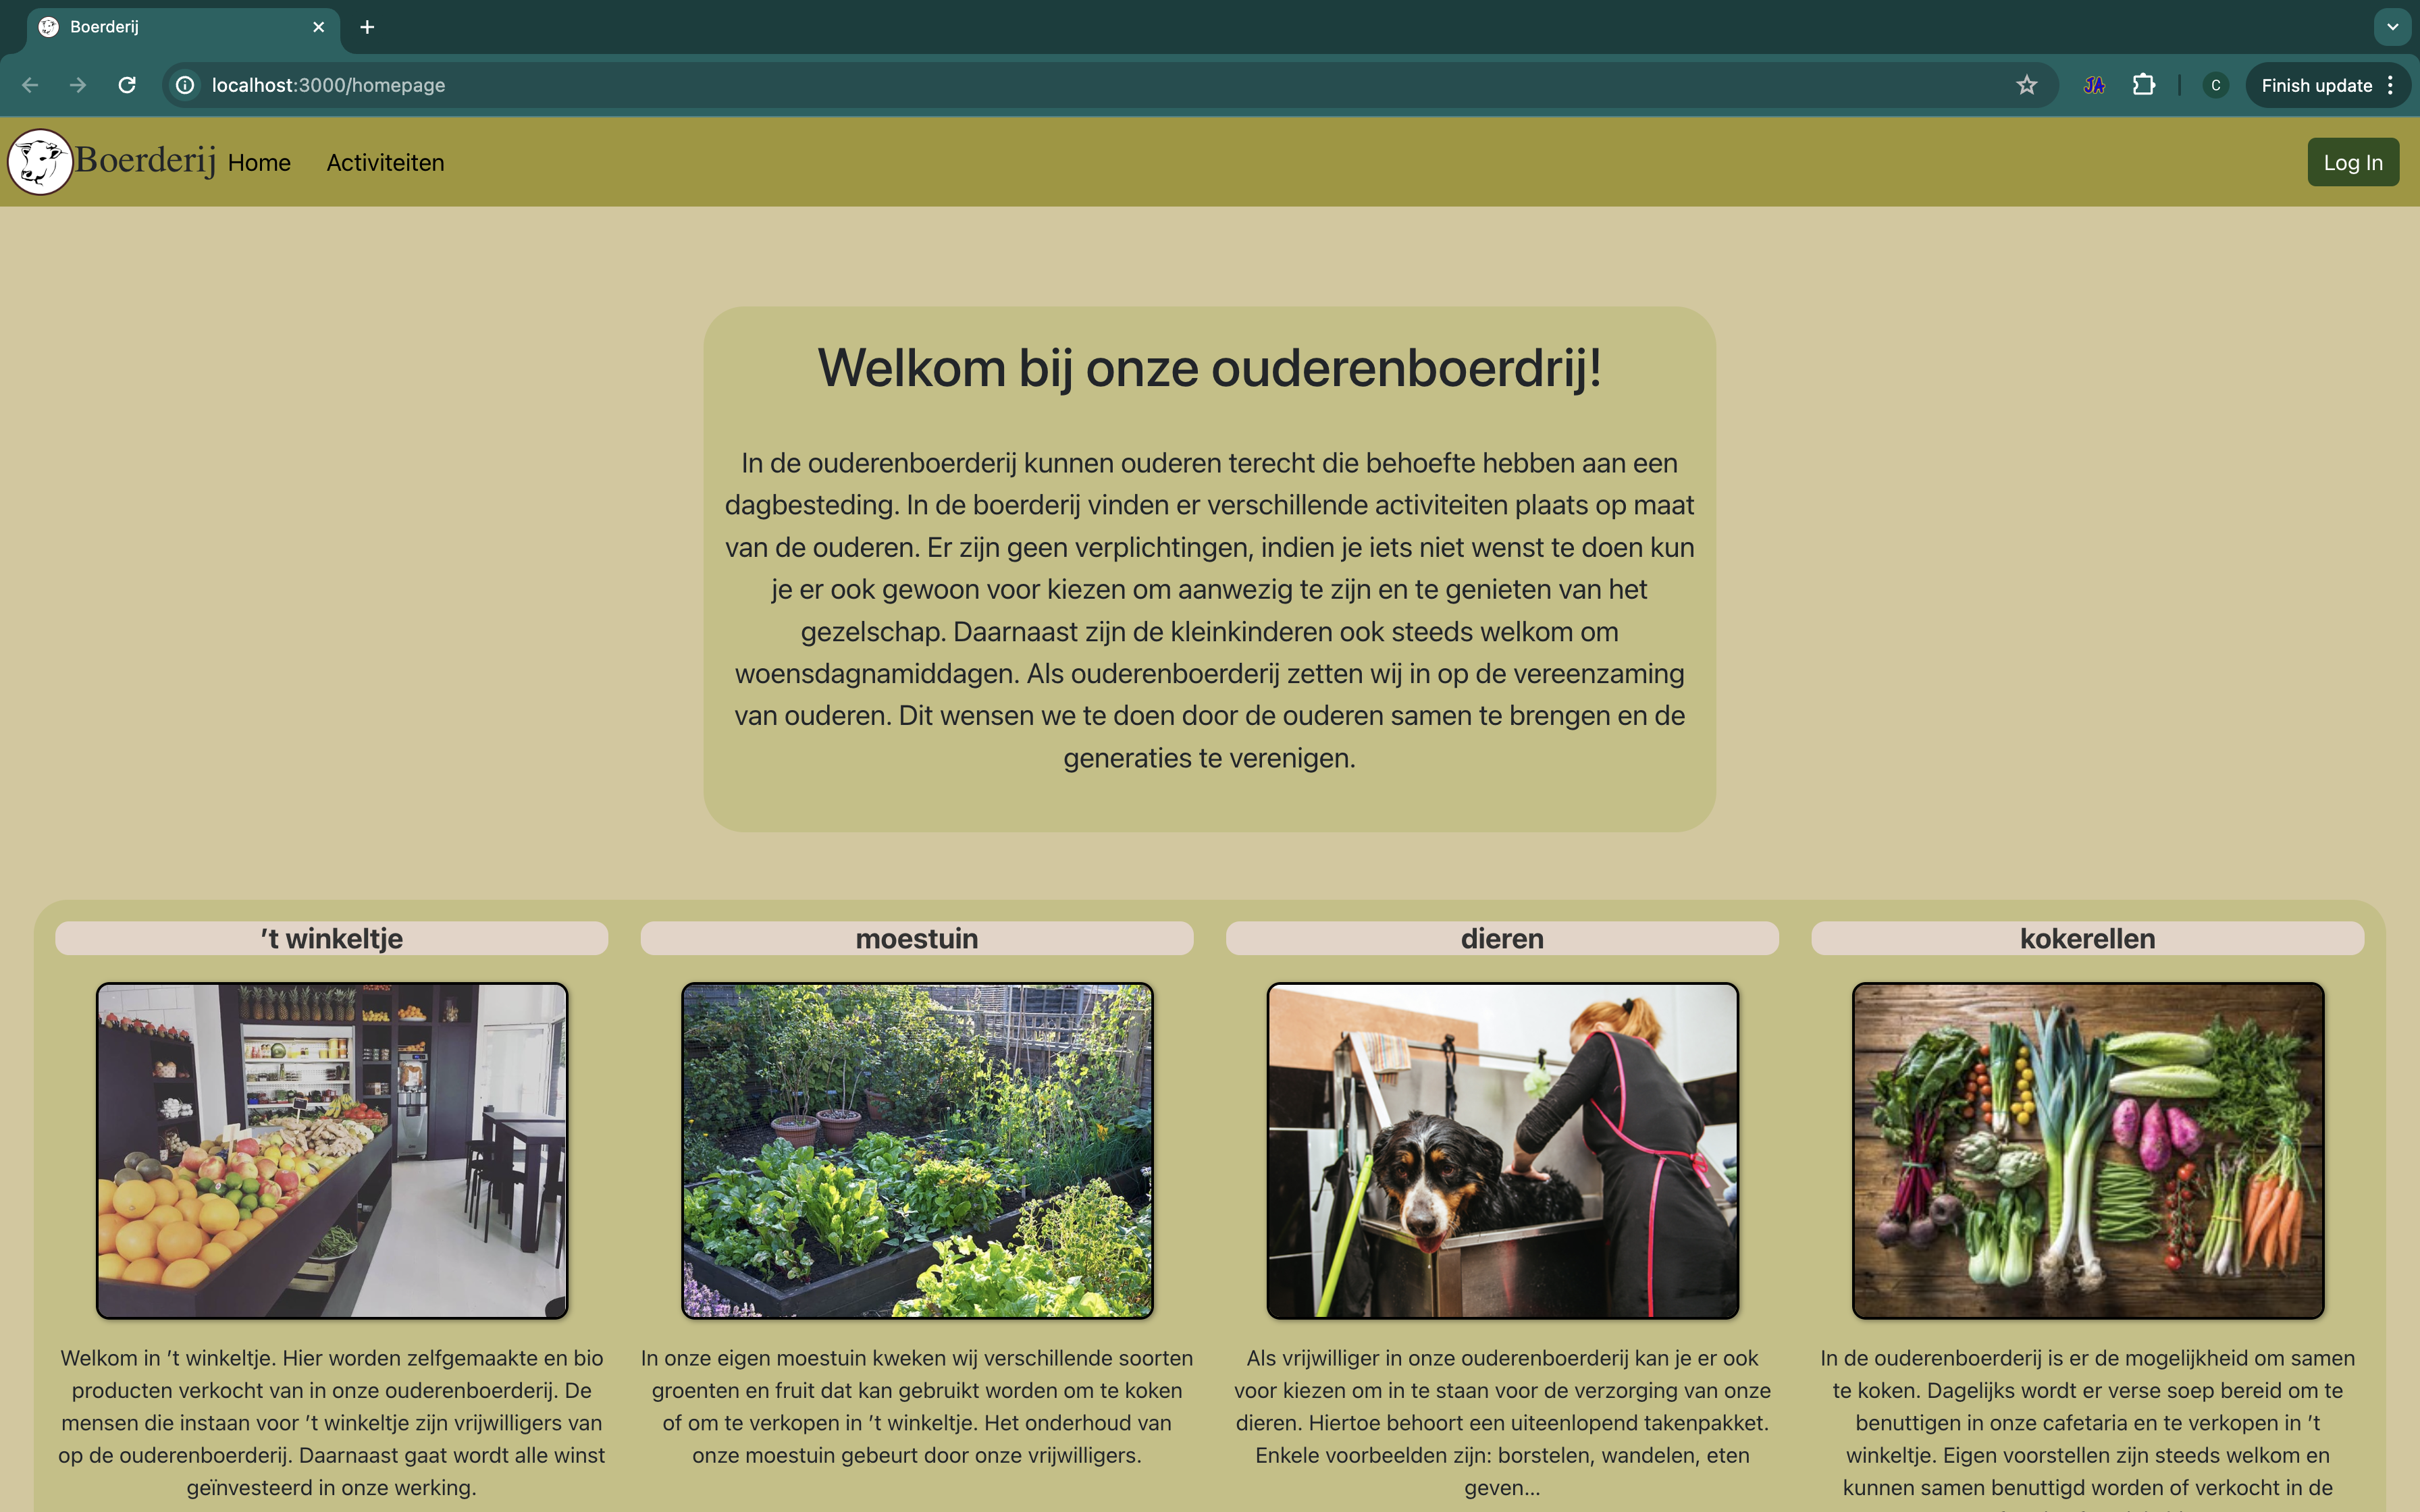
\includegraphics[width = 14cm]{Homescreen.png} 
    \caption{Homepagina} 
    \label{fig:home}
\end{figure}

Vanaf de homepagina kan de gebruiker zich inloggen of registreren. Na het inloggen krijgt de gebruiker toegang tot zijn profielpagina waar hij zijn gegevens kan aanpassen 

\begin{figure}[H]
    \centering	
    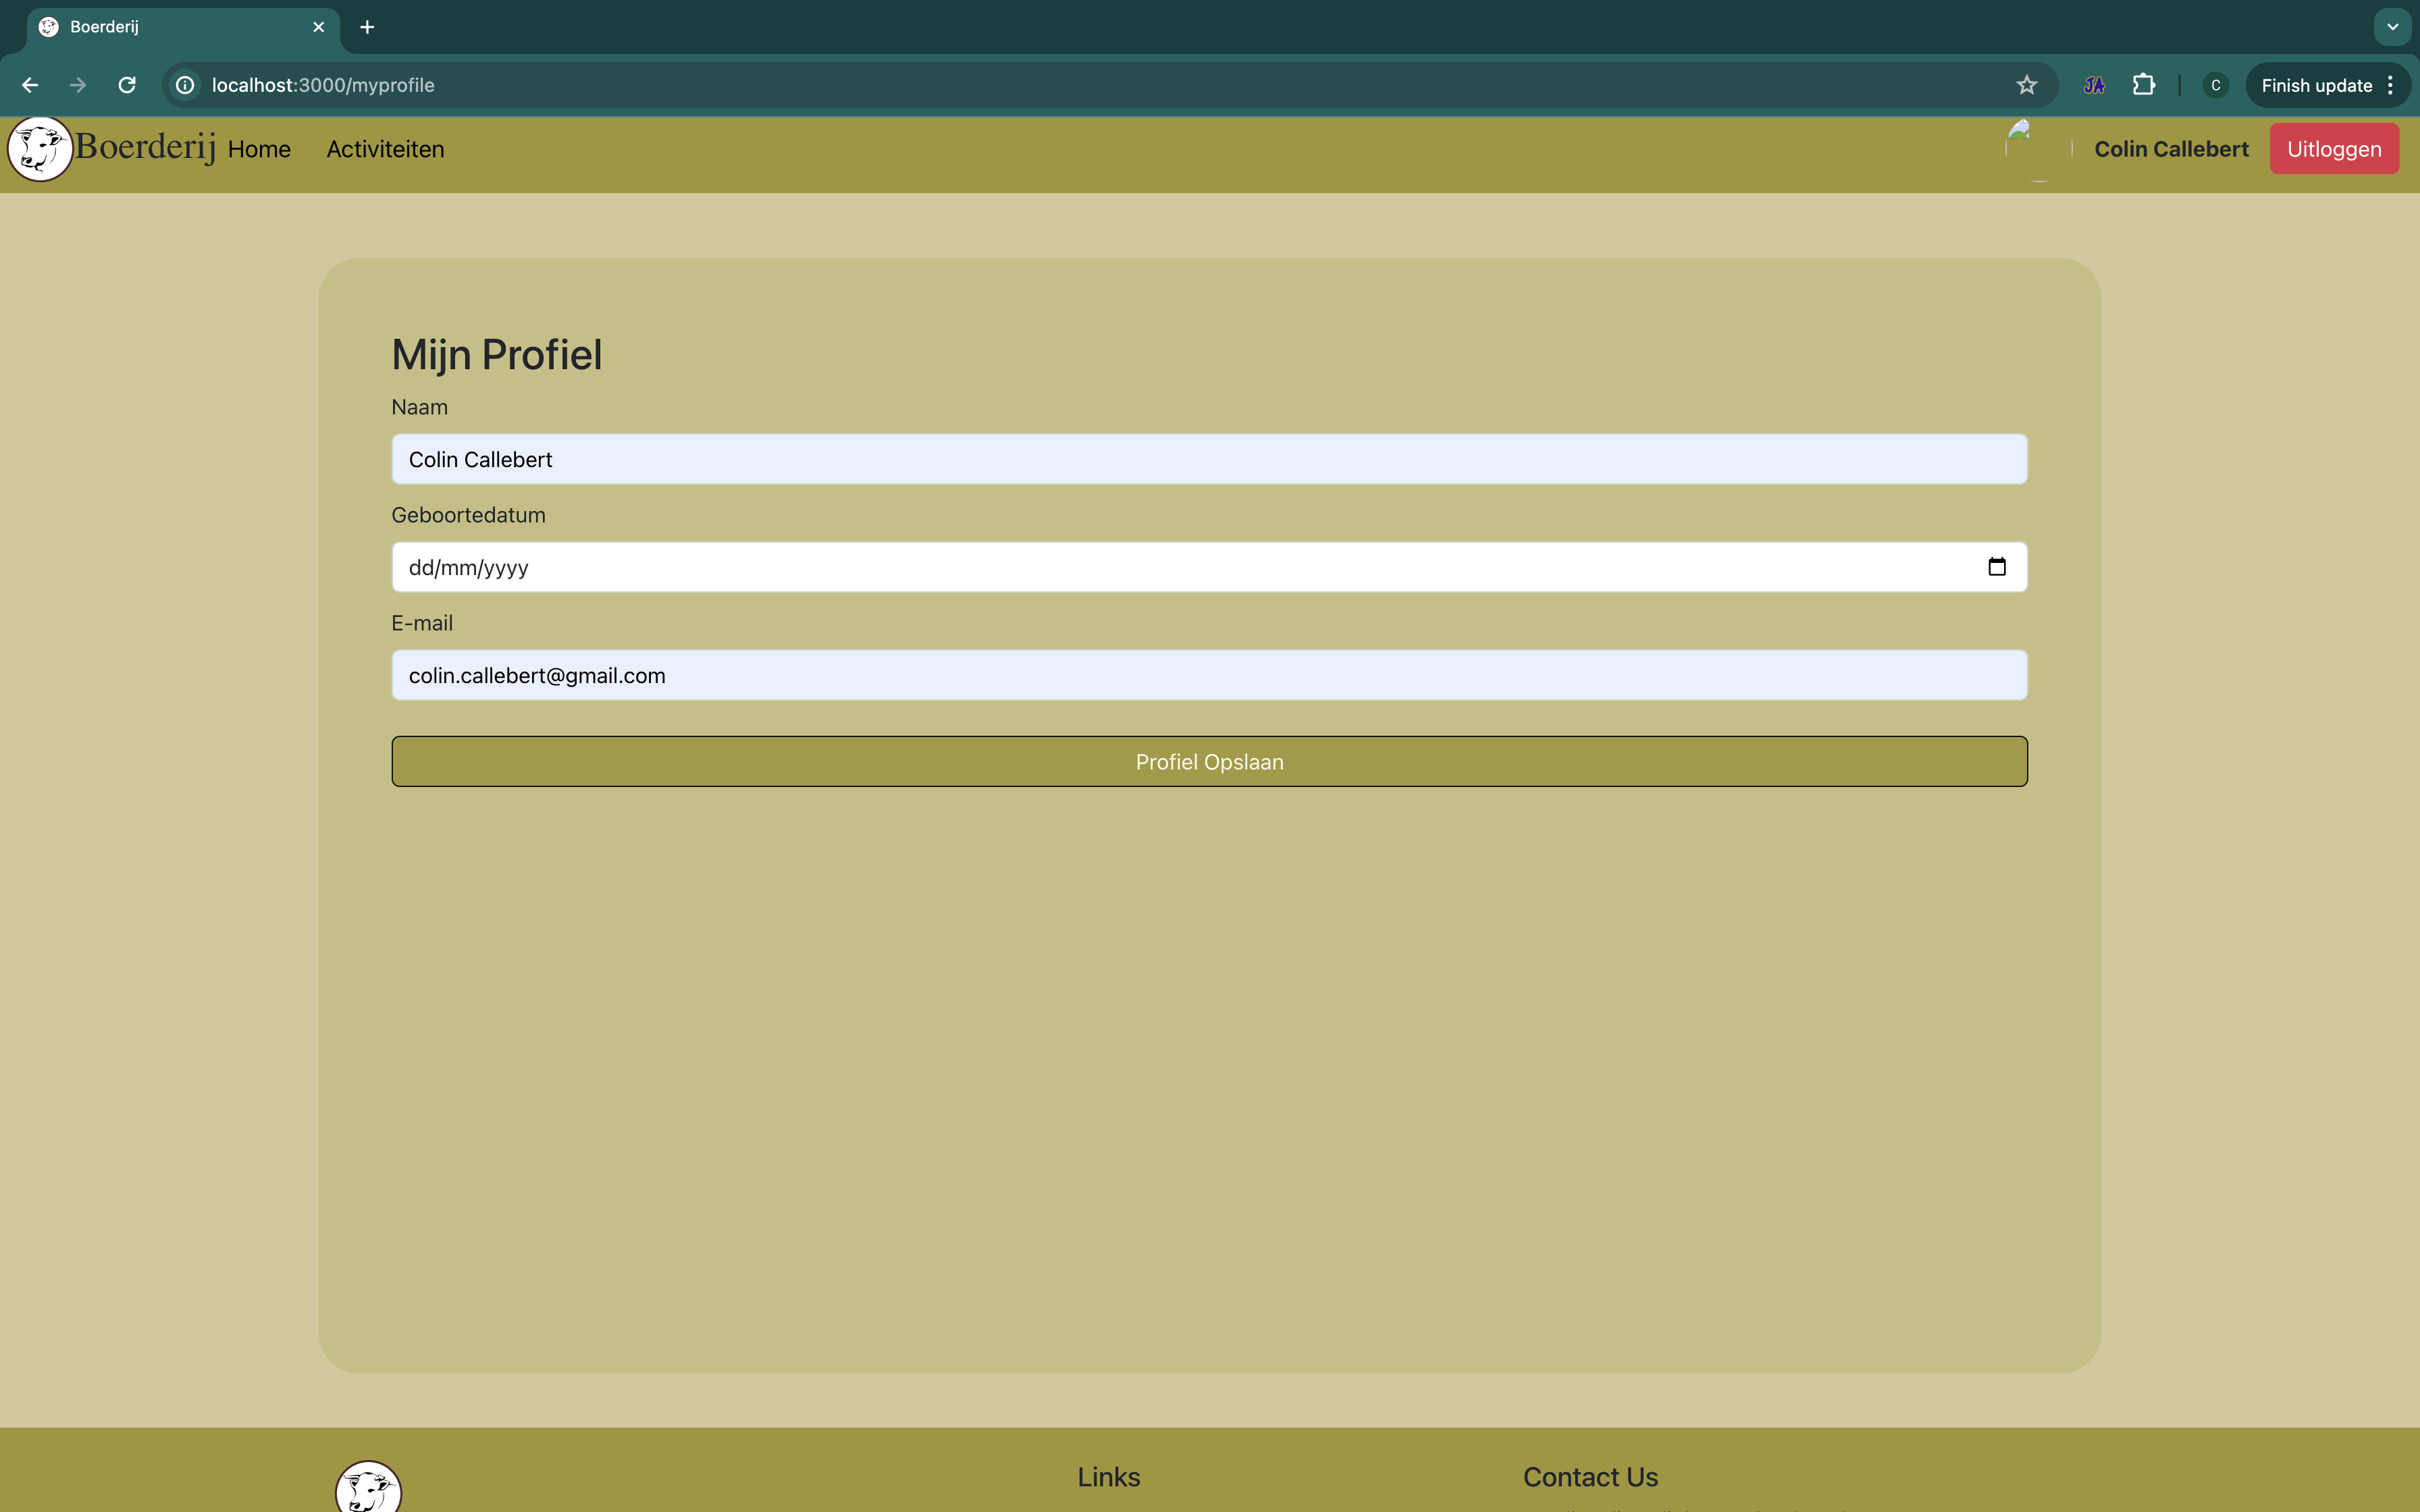
\includegraphics[width = 14cm]{Profiel.png} 
    \caption{Profielpagina} 
    \label{fig:profile}
\end{figure}

De gebruiker kan zich ook registreren voor activiteiten. De activiteiten worden weergegeven op de activiteitenpagina.

\begin{figure}[H]
    \centering	
    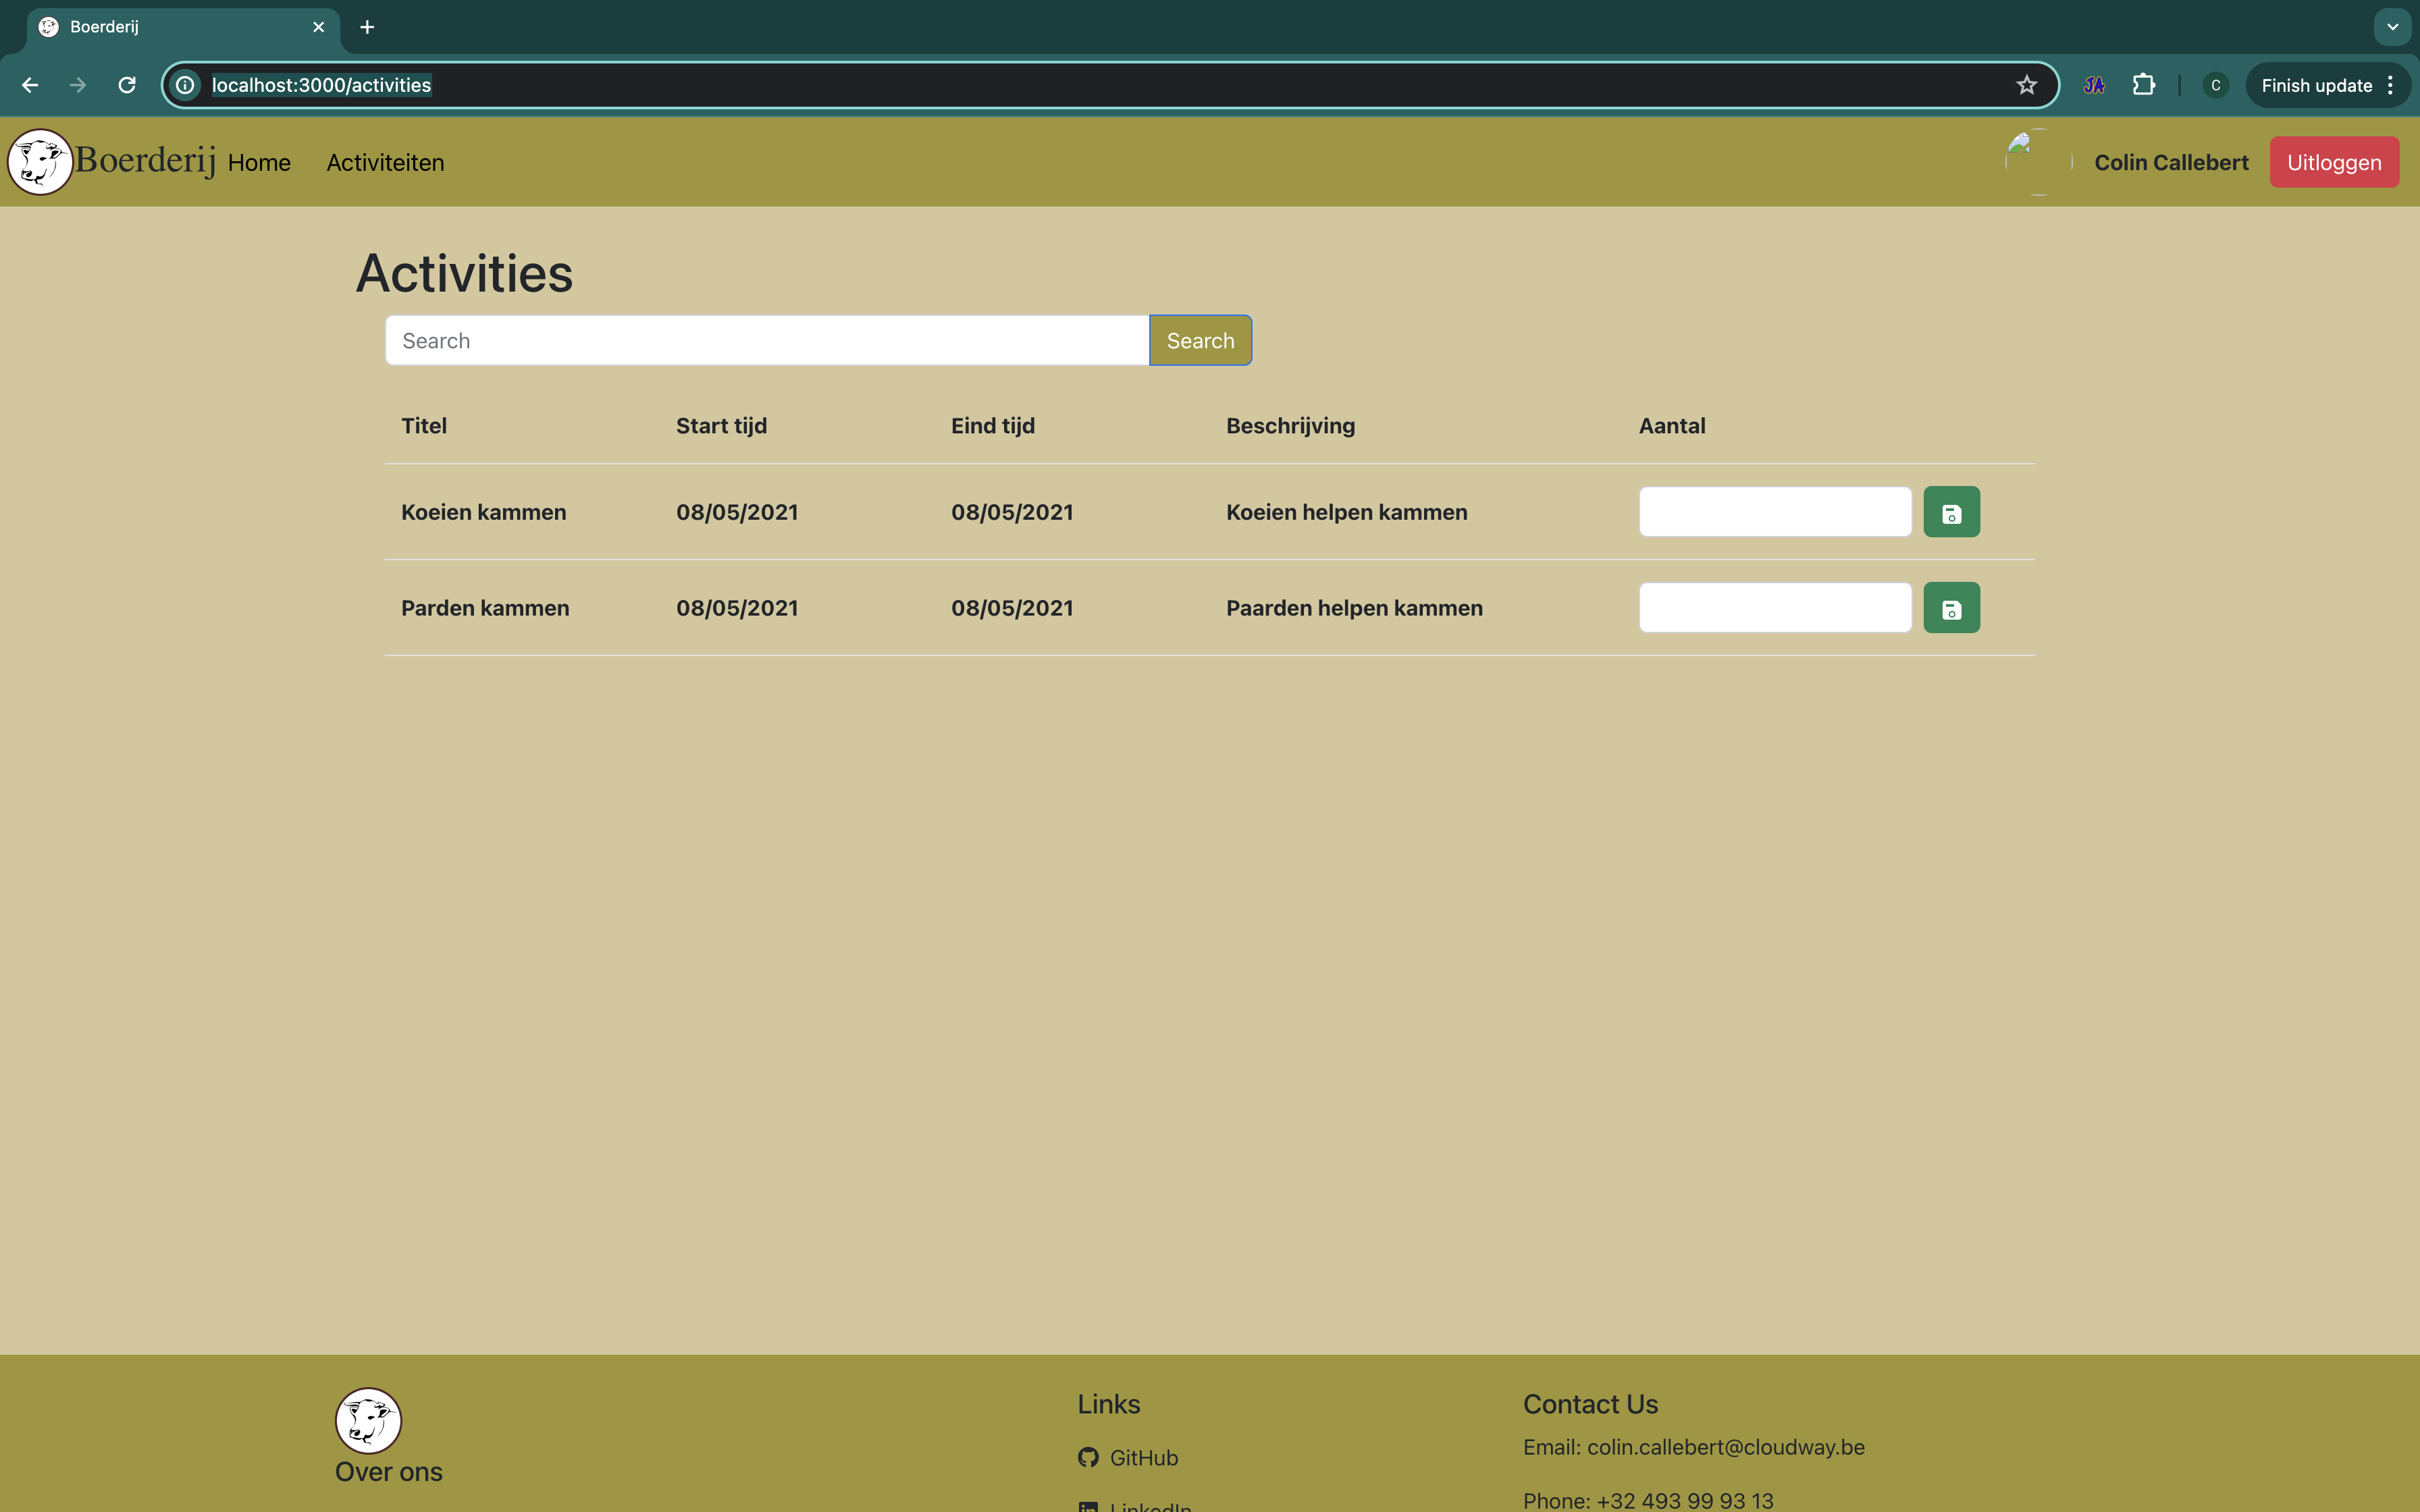
\includegraphics[width = 14cm]{Activiteiten.png} 
    \caption{Activiteitenpagina} 
    \label{fig:activities}
\end{figure}

De gebruiker kan zich inschrijven voor een activiteit door een aantal in te geven en op de knop te klikken.

\begin{figure}[H]
    \centering	
    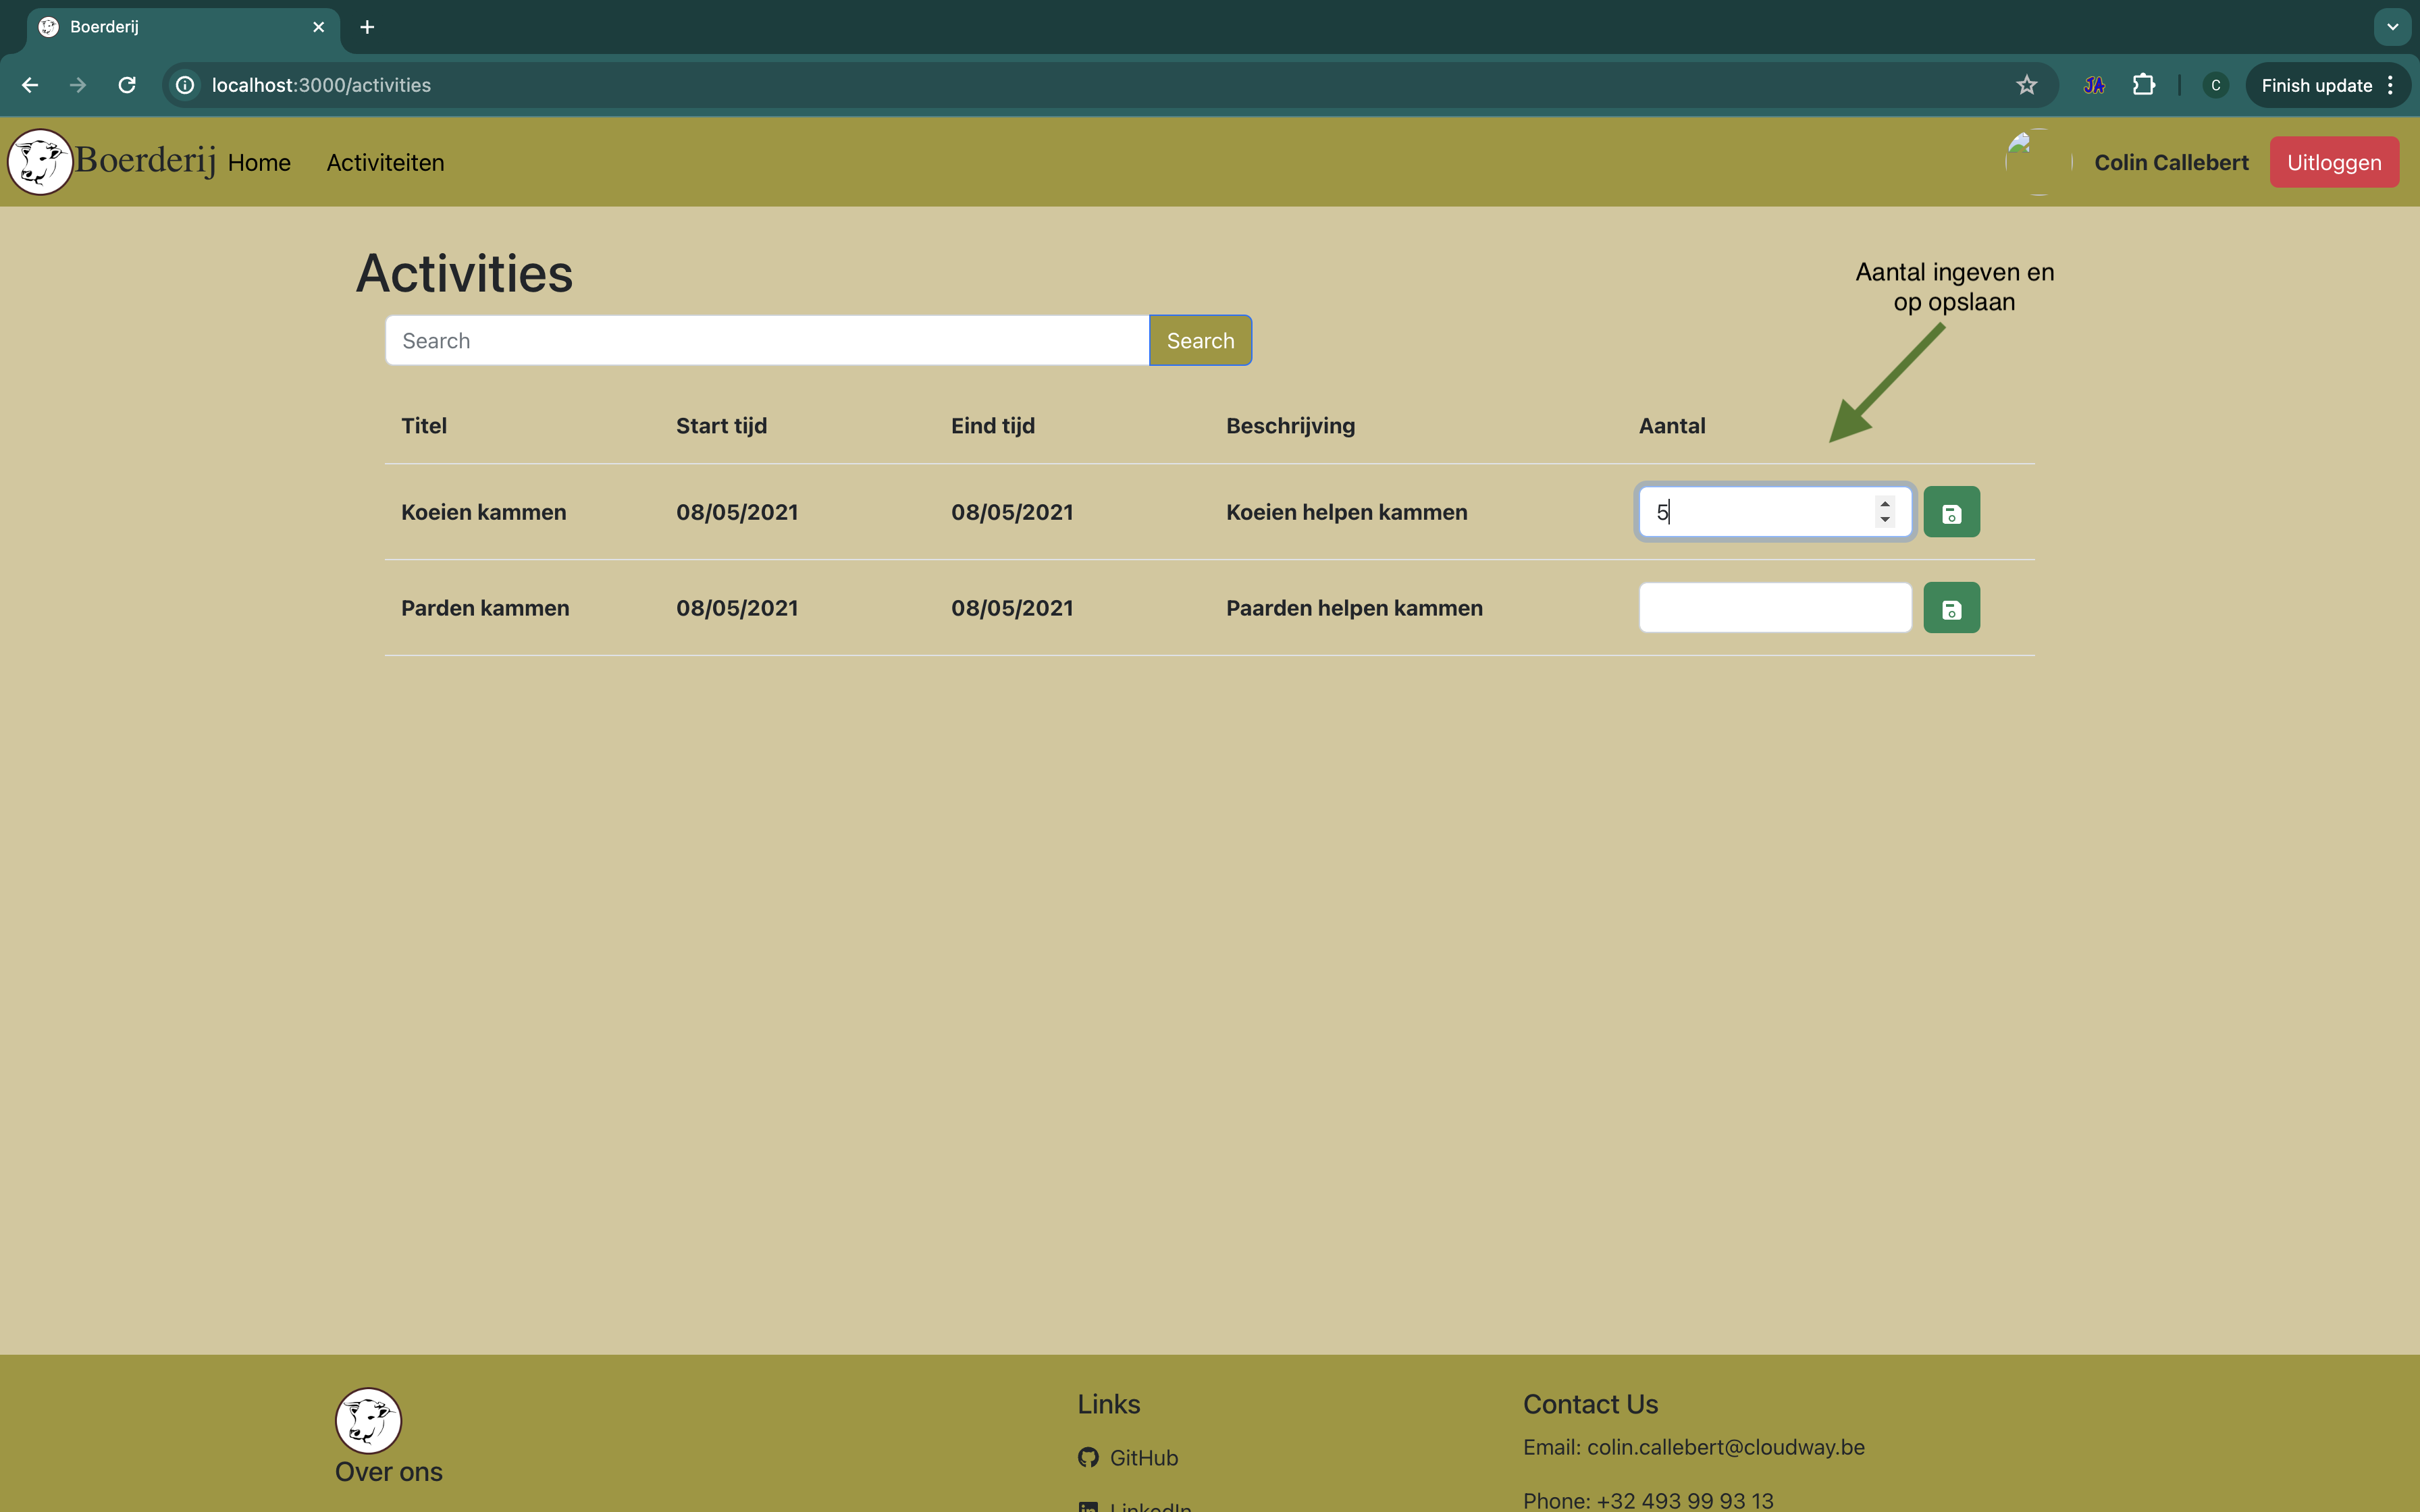
\includegraphics[width = 14cm]{ActiviteitAdd.png} 
    \caption{Inschrijven voor activiteit} 
    \label{fig:subscribe}
\end{figure}

Na het inschrijven voor een activiteit krijgt de gebruiker een bevestiging te zien.

\begin{figure}[H]
    \centering	
    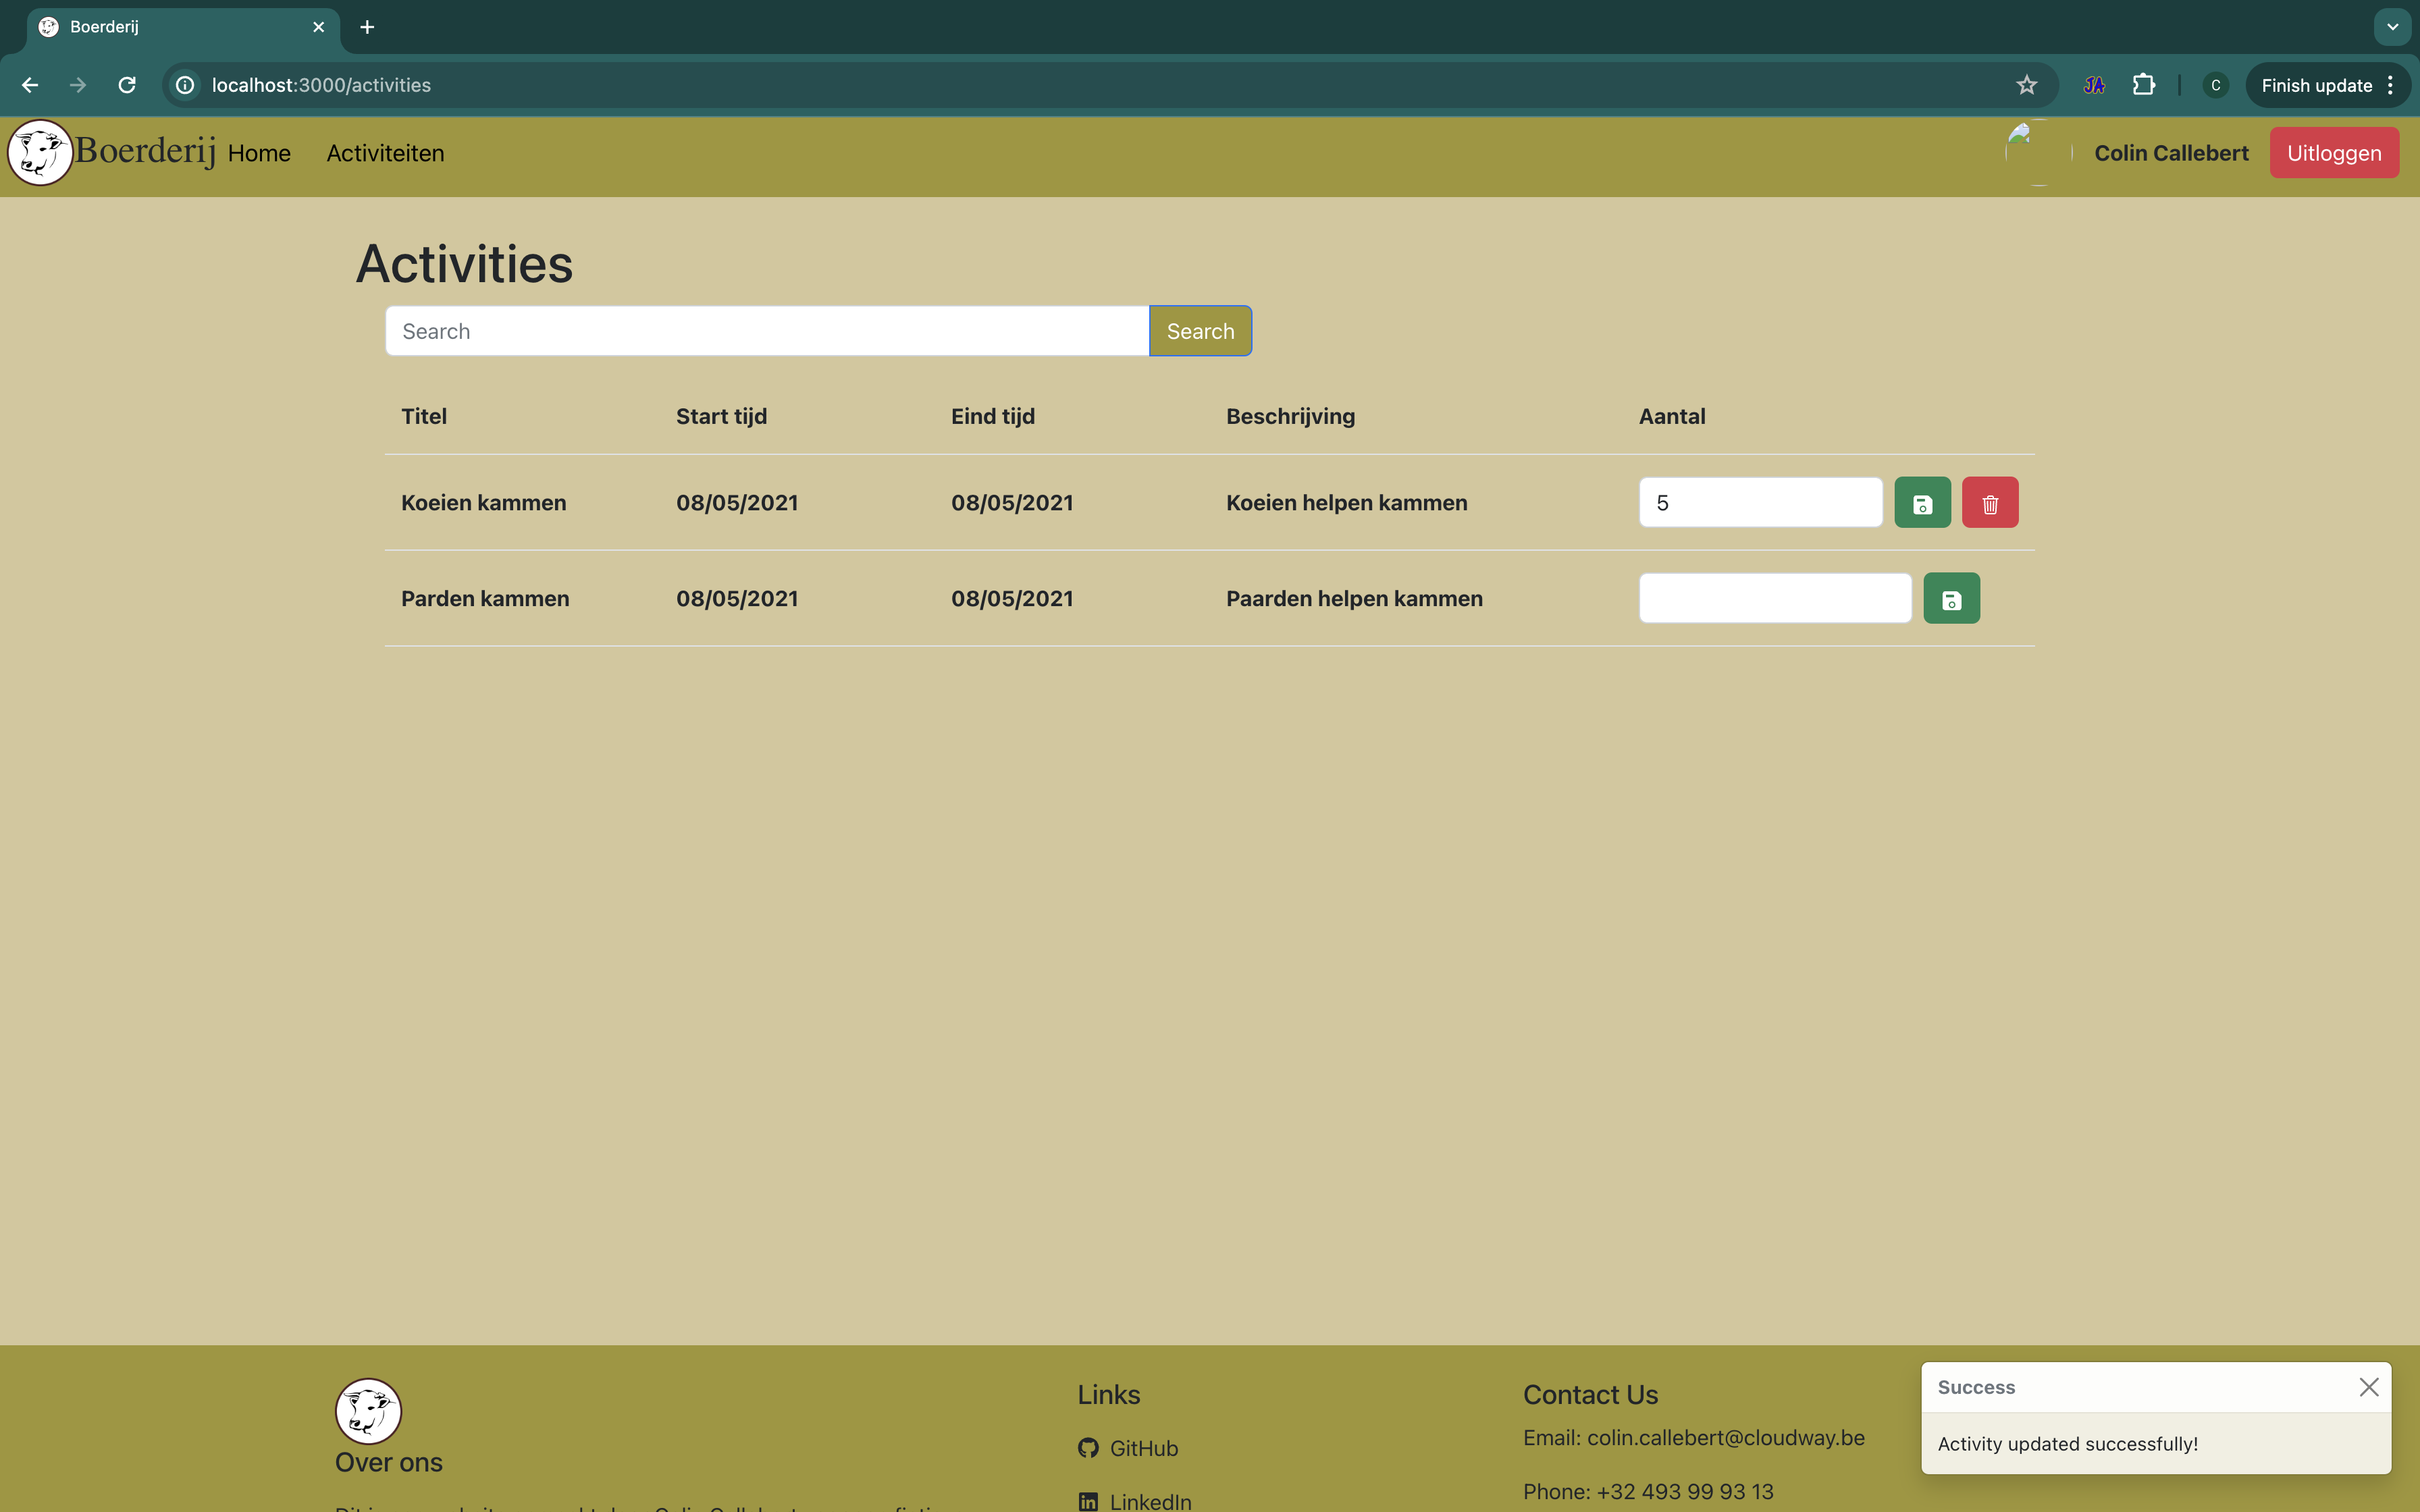
\includegraphics[width = 14cm]{ActiviteitAdd2.png} 
    \caption{Bevestiging inschrijving activiteit} 
    \label{fig:confirm}
\end{figure}

De gebruiker kan er ook voor kiezen om zich uit te schrijven voor een activiteit.

\begin{figure}[H]
    \centering	
    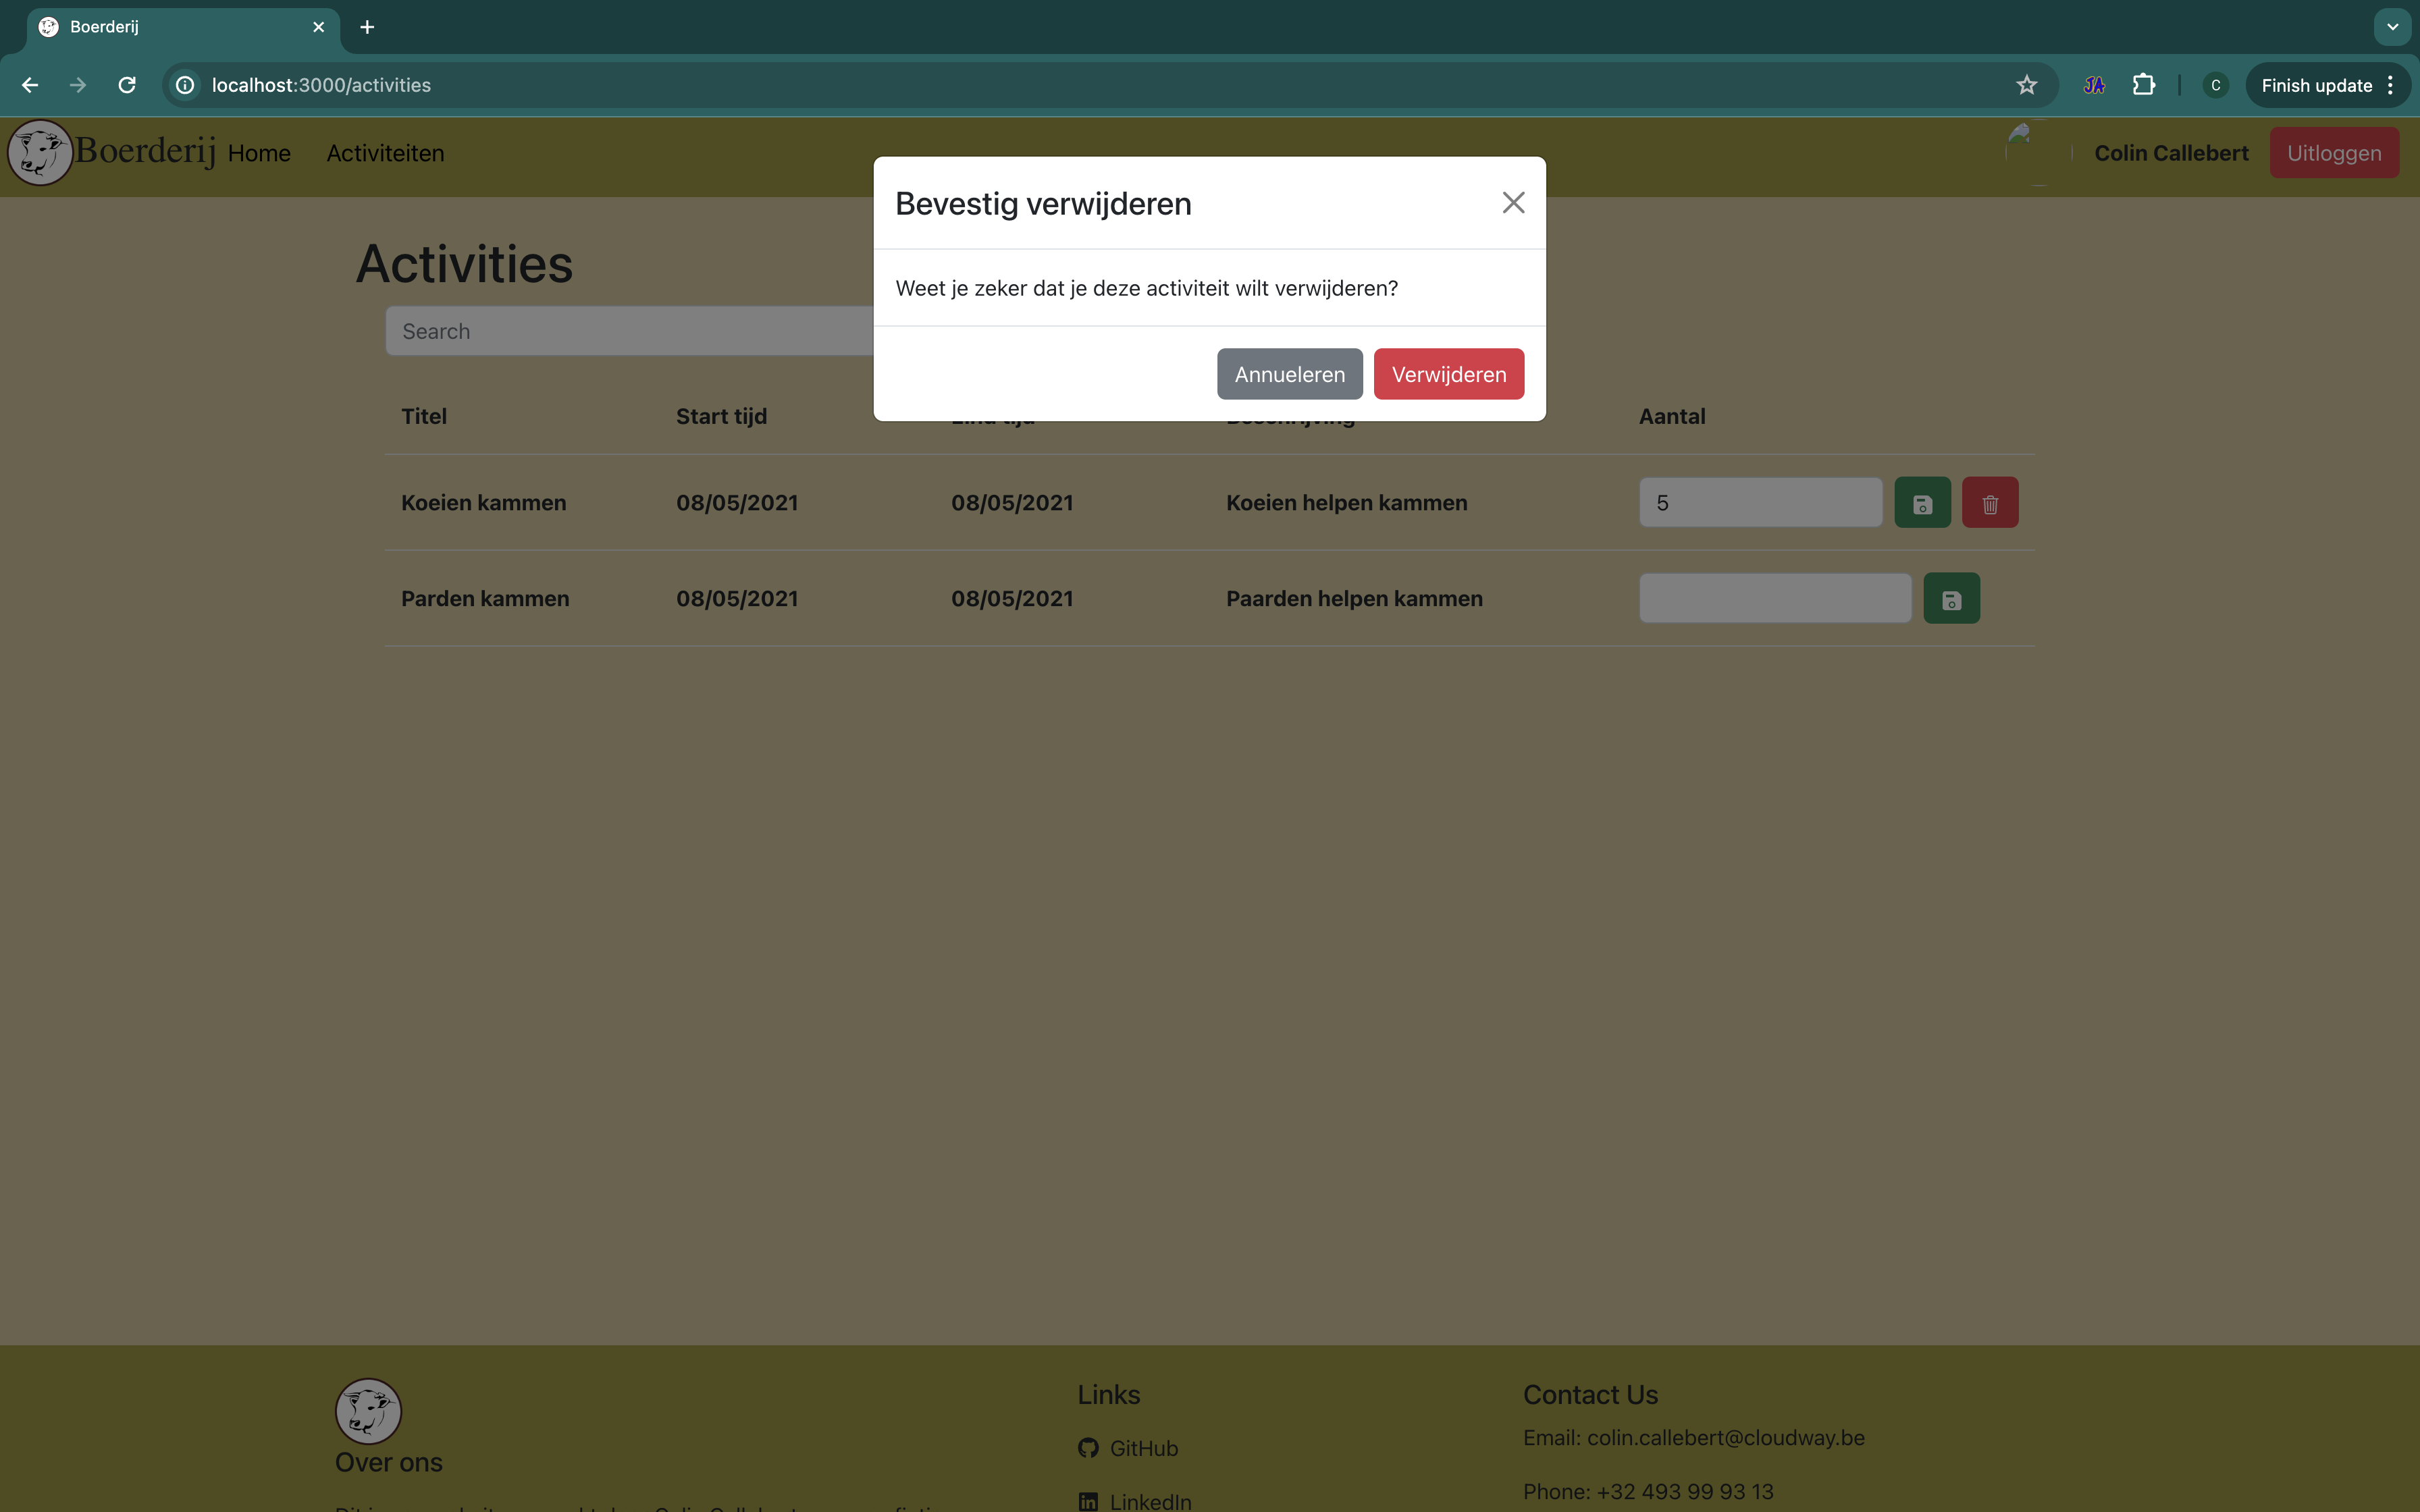
\includegraphics[width = 14cm]{ActiviteitRemove.png} 
    \caption{Uitschrijven voor activiteit} 
    \label{fig:unsubscribe}
\end{figure}

Deze versie biedt een goede basis voor de verdere ontwikkeling van de applicatie die dan opgesplitst kan worden in microservices.

Vervolgens wordt het monolithische ontwerp opgesplitst en herstructureerd naar drie afzonderlijke services, elk verantwoordelijk voor specifieke functionaliteiten. Deze aanpak stelt me in staat om de modulariteit, onderhoudbaarheid en schaalbaarheid van het systeem te verbeteren, terwijl ook de ontwikkeling en implementatie van nieuwe features wordt vergemakkelijkt.

